
%
% introduction.tex
% Copyright (C) 1995 by John Heidemann, <johnh@isi.edu>.
% $Id: demo2int.tex,v 1.1 1996/01/12 18:13:58 johnh Exp $
%

\chapter{Introduction}

\indent All is not well in cosmology. Approximately $80\%$ of the mass in the Universe exists in the form of dark matter, a mysterious entity of unknown origin and particle nature. The force of gravity mediates the only interactions between us and the ubiquitous dark matter. Through gravity, it pulls the strings of cosmic structure formation, explaining the formation and evolution of galaxies such as the Milky Way. Through gravity, dark matter also bends the path of light. 

Approximately 9 billion years ago, four photons were ejected from the quasar WFI2033-4723. Left to fly freely, a distance of roughly $100,000$ light years would separate them at the present time. Instead, we find the photons collected today on the primary mirror of the Hubble Space Telescope. The gravitational field of a massive galaxy and its surrounding dark matter, precisely aligned between us and WFI2033-4723, intervened to deflect light emitted from the distant quasar. The warping of space caused by the foreground galaxy is so extreme that several different paths connect the Hubble telescope with the background source, producing multiple images of the quasar at different positions on the sky. This phenomenon is referred to as strong gravitational lensing. Figure \ref{fig:lens2033} shows six examples of quadruply-image strong lenses, or \textit{quads}, including the system WFI2033-4723.

The direct coupling of light to mass through gravity in strong lenses provides a means of probing otherwise-undetectable dark matter structure. By extracting the information contained in the positions and magnifications of the multiple images in quads, we can measure the mass function and density profiles of dark matter halos scattered throughout the Universe. If the reigning cosmological theory of Cold Dark Matter (CDM) is correct, countless of these halos should litter the cosmos and produce gravitational lensing effects, while alternative theories predict that low-mass halos do not exist. A positive detection of low-mass dark matter halos through lensing would therefore confirm a central prediction of CDM, while a non-detection would potentially overthrow entire classes of particle physics models that predict a plethora of dark matter structure in the Universe. Either result would bring us one step closer towards understanding the nature of dark matter, one of the most confounding mysteries in modern cosmology. 

\begin{figure*}
	\centering
	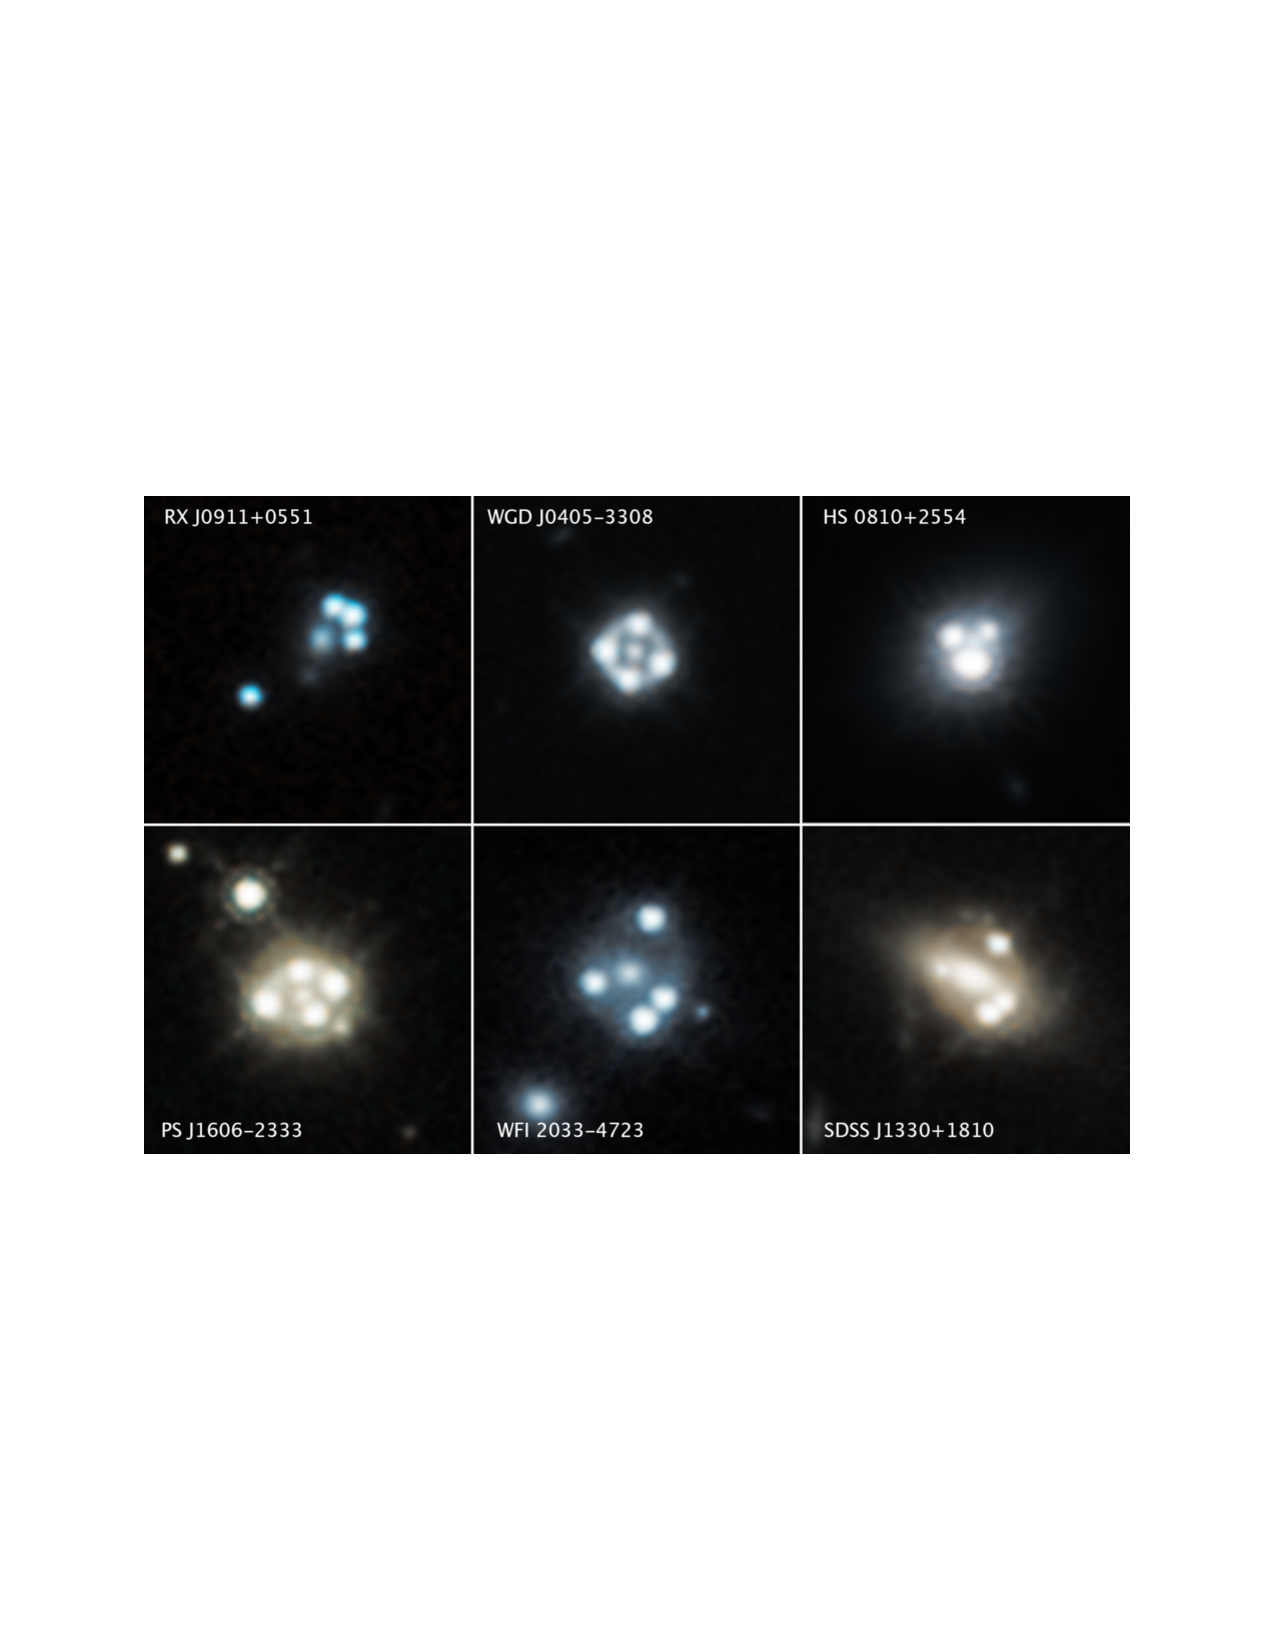
\includegraphics[clip,trim=2.5cm 8cm 2.5cm
	8.5cm,width=.95\textwidth,keepaspectratio]{./figures_introduction/lenses.pdf}
	\caption[Six images of strong gravitational lenses]{\label{fig:lens2033} Six quadruple-image strong gravitational lens systems imaged by the Hubble Space Telescope \cite{Nierenberg++19}. The main lensing galaxy is visible as the faint object encircled by four highly-magnified images of a background quasar. Image credit: NASA, ESA, A. Nierenberg (JPL) and T. Treu (UCLA)}
\end{figure*}	
In this dissertation, I describe research that constrains particle theories of dark matter with strong gravitational lensing. The following sections of this introduction set the stage for Chapters 2-6, which describe the development and implementation of a technique to constrain any dark matter model using the image magnifications from a sample of quads. Section 1.1 begins with a review of how the particle nature of dark matter drives structure formation in the Universe, and what aspects of structure formation lensing can constrain. Next, I review the basic theory connecting dark matter structure to lensing observables. 

\section{Structure formation and dark matter physics}
\indent Particle theories of dark matter predict the eventual collapse of an initially diffuse field of dark matter particles into gravitationally-bound halos through a mechanism called `violent relaxation' \cite{LyndenBell67}. The halo mass function, or the number of collapsed structures per unit mass, encodes information about when the first dark matter halos collapsed in the early Universe. Similarly, the density profiles of individual halos as a function of mass, the mass-concentration relation, depends on the hierarchical assembly history of dark matter halos through cosmic time, and the shape of the primordial matter power spectrum that seeded the growth of structure. 

Both the halo mass function and mass-concentration relation depend directly on the particle nature of dark matter. As a concrete example, consider two competing classes of dark matter models: Cold, and Warm Dark Matter (CDM and WDM, respectively). A quantity called the free-streaming length $\lambda_{\rm{FS}}$ distinguishes these two models. By definition, free-streaming effects are negligible in CDM, while in WDM scenarios the diffusion of dark matter particles out of potential wells in the early Universe wipes out small-scale density fluctuations. This diffusion process transforms a density field initialized with a scale-free power spectrum $P\left(k\right) \propto k^{n}$ into a density field with a truncated power spectrum around $k \sim k_{\rm{FS}} = \frac{2 \pi}{\lambda_{FS}}$. The characteristic length scale $\lambda_{\rm{FS}}$ can be approximated as the comoving distance a particle could have traveled before structure begins growing in earnest around the time of matter-radiation equality $t_{\rm{EQ}}$ \cite{Schneider++12} 
\begin{figure}
	\centering
	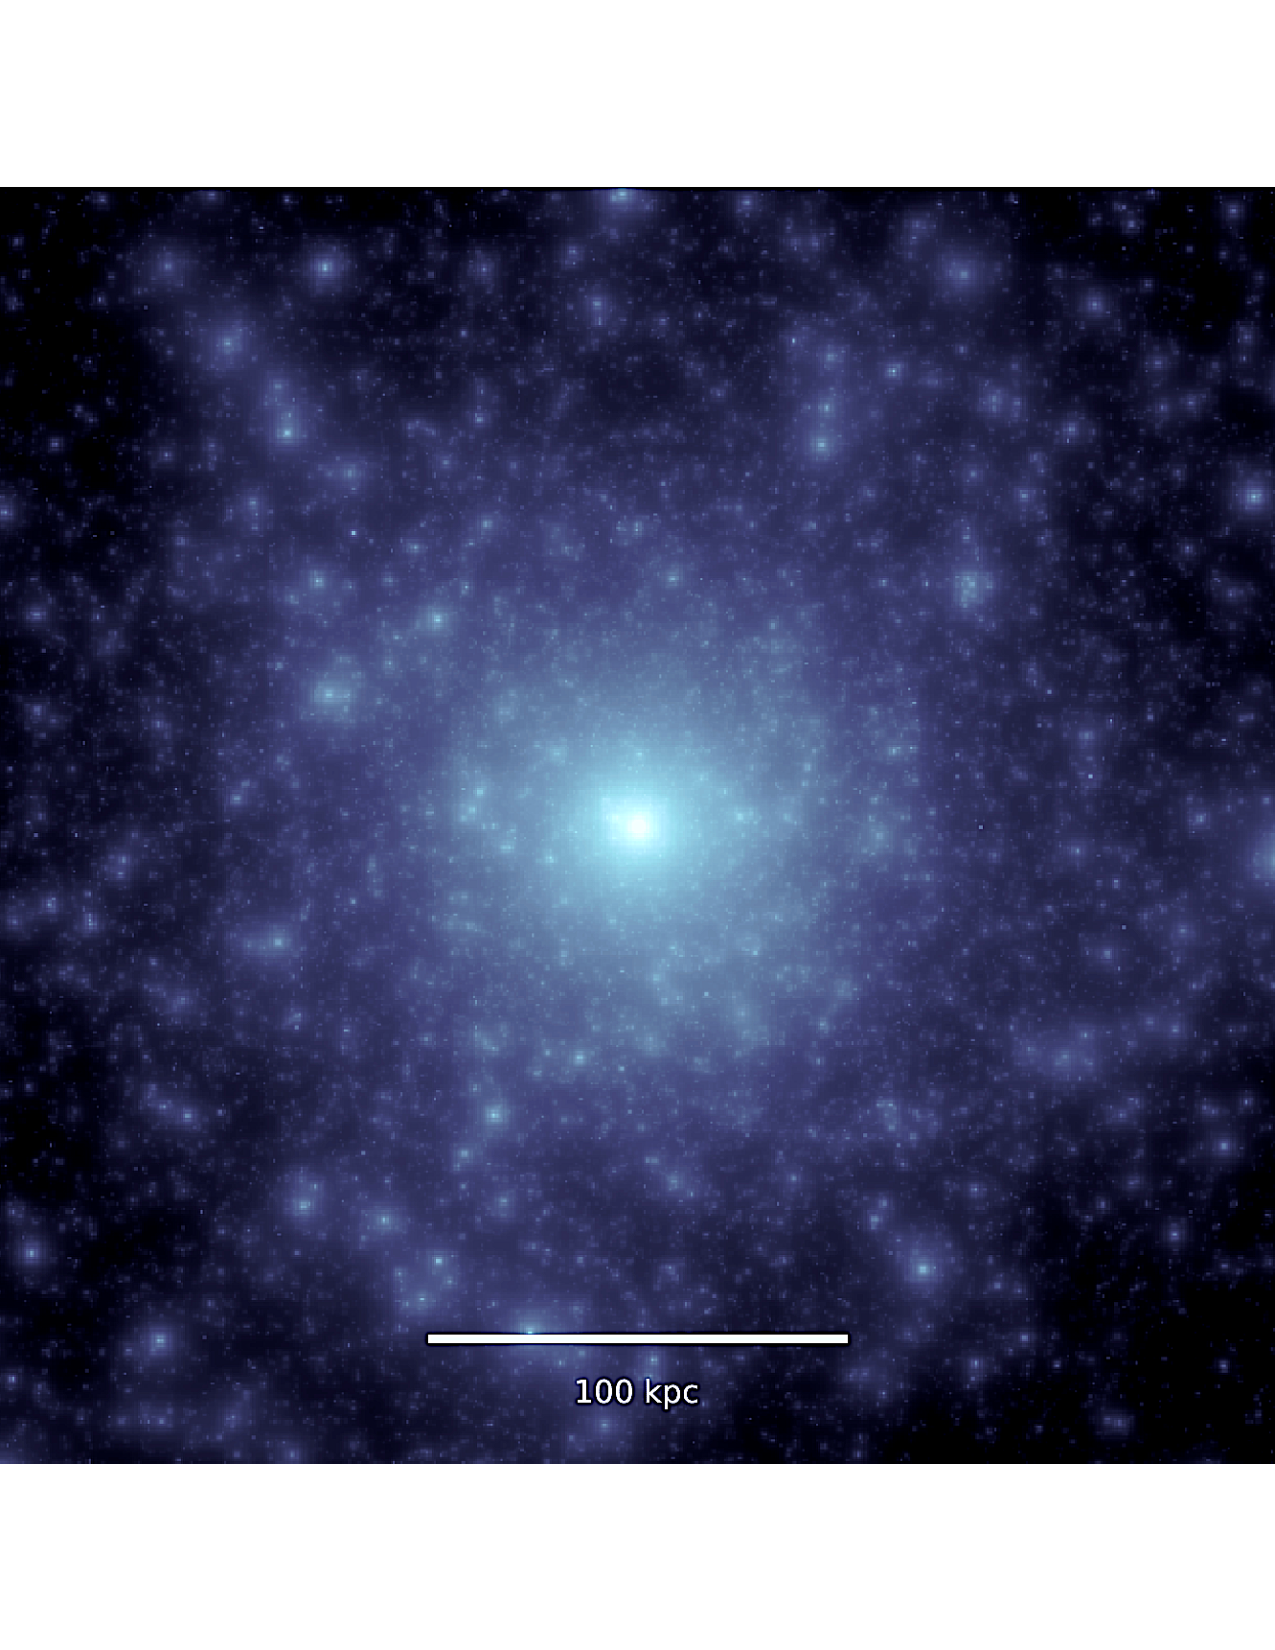
\includegraphics[clip,trim=0cm 0cm 0cm
	0cm,width=.49\textwidth,keepaspectratio]{./figures_introduction/CDMscreenshot_edited.pdf}
	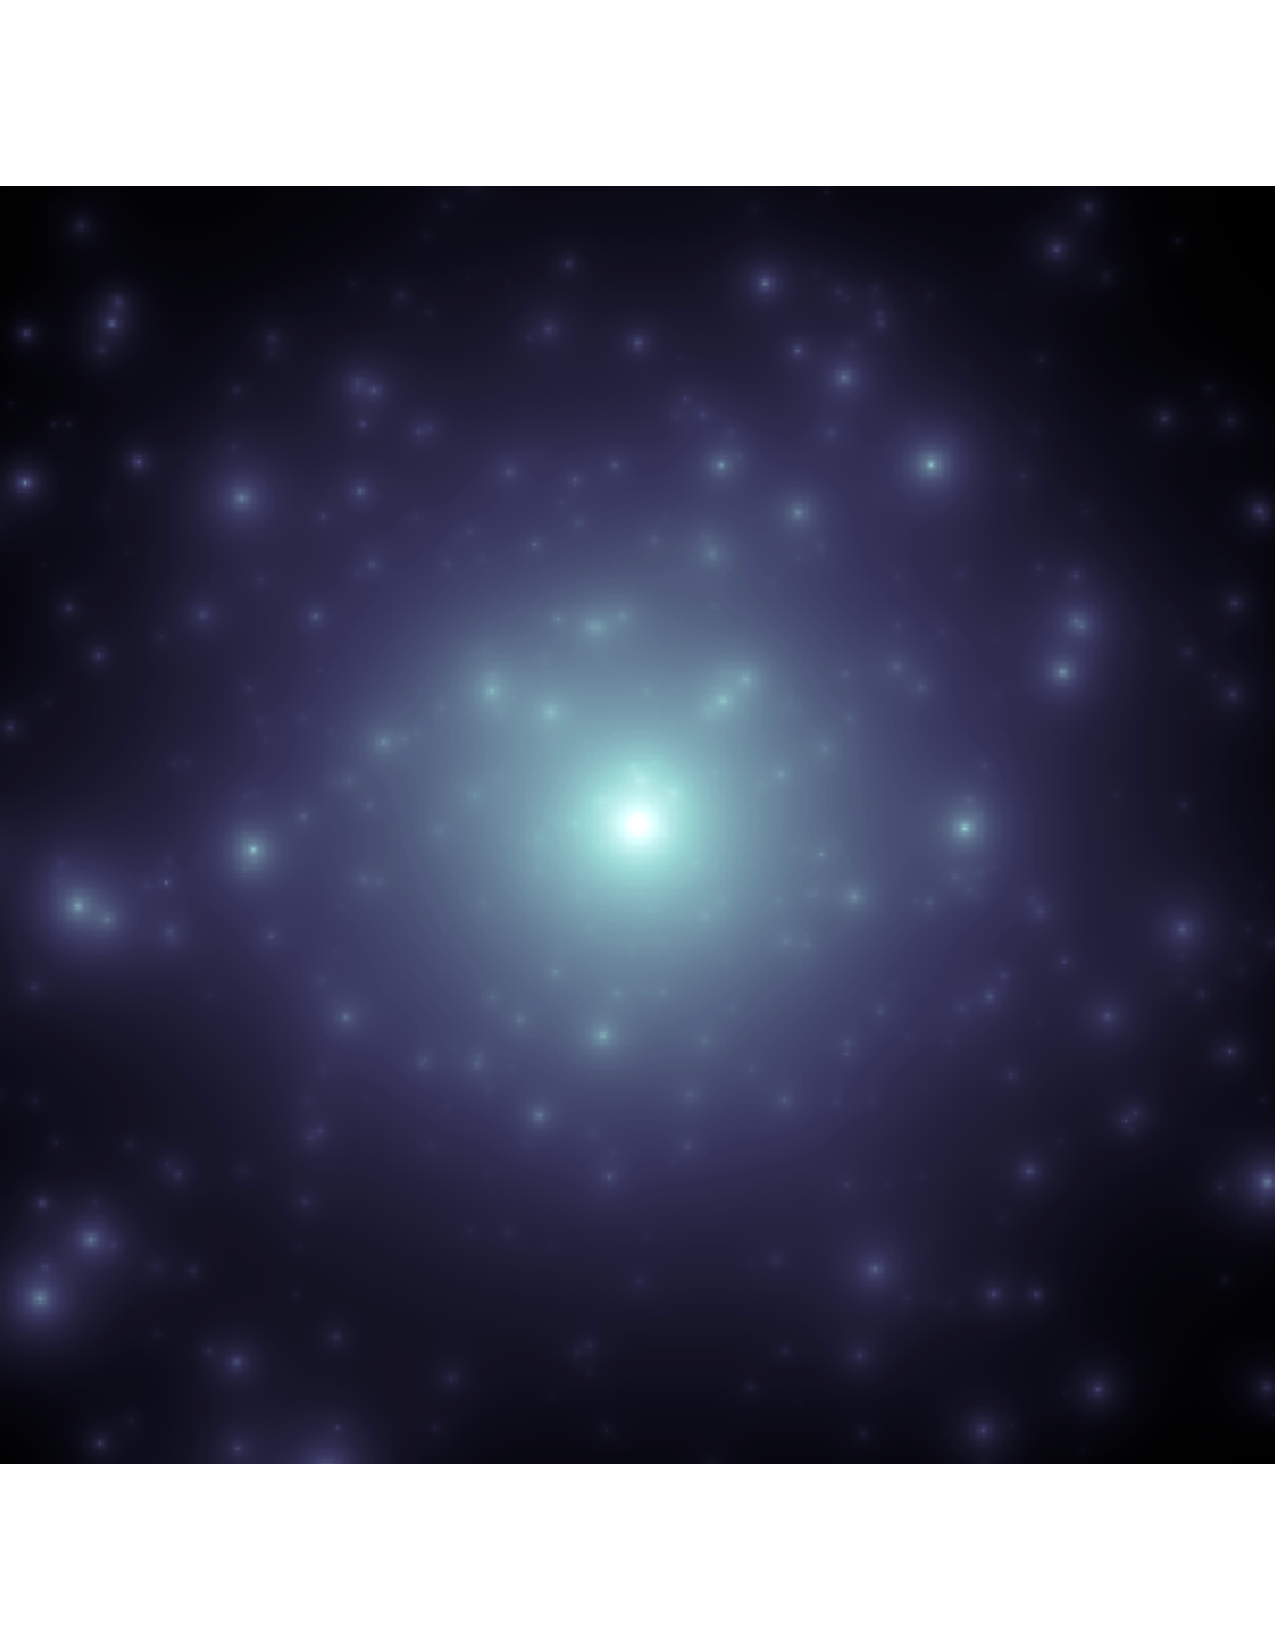
\includegraphics[clip,trim=0cm 0cm 0cm
	0cm,width=.49\textwidth,keepaspectratio]{./figures_introduction/WDMrealization_nobar.pdf}
	\caption[CDM and WDM subhalo populations]{\label{fig:wdmrealization} {\bf{Left:}} A realization of CDM substructure, with a scale-free subhalo mass function. {\bf{Right:}} A realization of WDM substructure corresponding to a $3.3 \rm{keV}$ thermal relic dark matter particle, which produces a turnover in the halo mass function around $10^8$ solar masses. }
\end{figure}

\begin{equation}
\label{eqn:freestreaming}
\lambda_{FS} \approx \int_{0}^{t_{\rm{NR}}} \frac{c dt}{a\left(t\right)} +  \int_{t_{\rm{NR}}}^{t_{\rm{EQ}}} \frac{v\left(t\right) dt}{a\left(t\right)} \approx r_{H}\left(t_{\rm{NR}}\right) \left(1 +\frac{1}{2} \log \frac{t_{\rm{EQ}}}{t_{\rm{NR}}} \right),
\end{equation}
where the particle has speed $c$ before becoming non-relativistic at time $t_{NR}$, $r_H \left(t_{\rm{NR}}\right)$ is the comoving horizon size at $t_{\rm{NR}}$, $a\left(t\right)$ is the cosmological scale factor, and $v\left(t\right)$ represents the average velocity distribution of the dark matter particles\footnote{This expression assumes that the particles become non-relativistic before $t_{\rm{EQ}}$, and uses the fact that $a\left(t\right)\propto t^{\frac{1}{2}}$ before $t_{\rm{EQ}}$.}. 

The effects of free-streaming manifest in structure formation in two ways: First, erasing small-scale power at early times eliminates the small-scale density fluctuations in the primordial matter density field that would collapse into the smallest dark matter halos. This suppression of small-scale power results in a turnover in the halo mass function at a certain mass scale that is proportional to the $k_{\rm{FS}}^{-3}$ \cite{AvilaReese++01,Schneider++12,Lovell++14}. Second, because low-mass halos collapse first in hierarchical structure formation scenarios, eliminating the smallest halos delays the onset of structure formation. As the central density profile of a dark matter halo reflects the background density of the Universe at the time of collapse, delaying structure formation suppresses the central density of dark matter halos, with effects extending over an order of magnitude in mass above the free-streaming scale \cite{Navarro++96,Bose++16}. These structure formation arguments apply to both isolated halos in the field, and subhalos of the $10^{13}$ solar mass host dark matter halos that contain early-type galaxies \cite{Gavazzi++07}. A CDM and a 3.3 keV thermal relic WDM subhalo population are shown in the left and right panels of Figure \ref{fig:wdmrealization}, respectively. 

The dependence of $\lambda_{FS}$ on features such as $t_{NR}$ and $v\left(t\right)$ links the free-streaming length of the dark matter to the formation mechanism and velocity distribution of the dark matter particle(s). As the halo mass function and mass-concentration relation depend on the free-streaming length, it follows that constraining the halo mass function and halo density profiles can be cast as a constraint on fundamental dark matter physics determining $t_{NR}$ and $v\left(t\right)$. Notice, however, that none of the previous discussion depends on a particular choice of dark matter model; properties such as the free-streaming length can be computed for practically any model in the literature, a fact that illustrates the power and broad scope of structure formation arguments. For example we can rule out neutrinos, thermal relics with mass $< 2 \rm{keV}$, and sterile neutrinos produced via Higgs decay with a mass of $7 \rm{keV}$ \cite{Viel13,AbazaijanKusenko19} making up 100$\%$ of the dark matter, as the free-streaming lengths corresponding to each these models precludes the formation of galaxies such as the Milky Way. 

In order to constrain dark matter models through structure formation arguments, one requires a method to detect, and measure the mass of, dark matter halos. One approach uses the fact that galaxies are believed to reside inside dark matter halos, so luminous structure, such as dwarf galaxies, therefore traces the underlying dark matter halos. Unfortunately, this approach becomes increasingly difficult below $10^9$ solar masses, as not every dark matter halo on sub-galactic mass scales hosts a visible galaxy. More generally, uncertainties stemming from astrophysics on sub-galactic scales can sometimes be larger that the differences between the dark matter models of interest \cite{Nierenberg++16}. While recent advances in this field make considerable progress towards appropriately dealing with these complications \cite{Nadler++19}, the use of luminous matter to trace small-scale dark matter structure is, at present, confined to the Milky Way. A second technique to probe small-scale structure in the Universe relies on the flux power spectrum of the Lyman-$\alpha$ forest at $z \sim 5$, which under certain assumptions can be used as a proxy for the matter power spectrum \cite{Viel13,Irsic++17}. The promise of this method must be weighed against the systematic uncertainties associated with the thermodynamics of the Lyman-$\alpha$ forest at high redshift, which can mimick the suppression of small-scale power in WDM scenarios \cite{Garzilli++19}. 

Strong gravitational lensing by galaxies offers an alternative, more direct probe of dark matter structure on scales below $10^8$ solar masses. Lensing couples only to gravity, and therefore circumvents the challenges associated with using baryonic matter to trace the underlying dark matter. In the next section, I review the formalism connecting lensing observables to populations of dark matter halos along the entire line of sight, from the observer to the source. 

\section{Strong lensing signatures of dark matter halos}
\indent General relativity relates the deflection angle of a light ray to the mass distribution of a massive structure, dark or luminous. When the distances scales between the observer, lens, and source are much greater than the physical extent of the lensing mass distribution, the effect of a massive deflector can be approximated as a single sharp deflection in the plane of the lens, the `thin lens' approximation. Defining $\Sigma$ as the projection of a deflector's three dimensional density profile onto the plane of the lens, the deflection angle is given by \cite{BlandfordNarayan86,Schnedier1997}
\begin{equation}
\label{eqn:defangle}
\vec{\alpha}\left(D_{\rm{d}} \vec{\theta}\right) = \frac{4G D_{\rm{d}}}{c^2} \int \frac{\left(\vec{\theta} - \vec{\theta}^{\prime}\right) \Sigma\left(D_{\rm{d}}\vec{\theta}^{\prime}\right)}{|\vec{\theta} - \vec{\theta}^{\prime}|^2} d^2 \vec{\theta^{\prime}}. 
\end{equation}
For multiple deflectors in a single lens plane, the cumulative effect is a linear superposition of their individual deflection angles $\vec{\alpha}$. 

A strong lens system will include both subhalos associated with the host dark matter halo of the lensing galaxy, and field matter halos distributed along the entire line of sight. Incorporating line of sight halos requires multi-plane ray tracing equation, which maps an angular coordinate on the sky $\vec{\theta_1}$ to an angular coordinate on the source plane $\vec{\theta_s}$. The ray tracing equation is given by \cite{BlandfordNarayan86}
\begin{equation}
\label{eqn:raytracingintro}
\vec{\theta_s} = \vec{\theta_1} - \frac{1}{D_{\rm{s}}} \sum_{i=1}^{s-1} D_{\rm{is}}{\vec{\alpha_{\rm{i}}}} \left(D_{\rm{i}} \vec{\theta_{\rm{i}}}\right),
\end{equation} 
where the net deflection angle from all halos at the $i$th lens plane can be computed with Equation \ref{eqn:defangle}, $D_{\rm{ij}}$ is the angular diameter distance from the $i$th lens plane to the $j$th, and subscript $s$ identifies the source plane. Equation \ref{eqn:raytracingintro} is a recursive equation for the net deflection angles at various lens planes, coupling deflections produced by halos at different distances. Equation \ref{eqn:raytracingintro} describes a physical process similar to viewing an image through multiple magnifying glasses in series. 

Equation \ref{eqn:raytracingintro} maps a single coordinate on the sky to a single coordinate on the source plane, determining where images appear to the observer. As gravitational lensing conserves surface brightness \cite{MisnerThorneWheeler}, the (de)magnification of the lensed images is proportional to the ratio of areas in the image and source planes given by the inverse determinant of the jacobian $\left(\det \frac{\partial \vec{\theta_s}}{\partial \vec{\theta_1}}\right)^{-1}$. While the full expression for the lensing jacobian in the general multi-plane framework (see \cite{BlandfordNarayan86}) is long and not particularly illuminating, the key point is that the magnification of an image depends non-linearly on derivatives of the lensing deflection angle. Image magnifications are therefore highly localized probes of the mass distribution along the line of sight to strong lenses. While the exact level of perturbation to an image magnification depends on the size of the background source, the mass of the halo, and the position of the image relative to the critical curve, a dark matter halo as diminutive as $10^7 M_{\odot}$ near a lensed image can induce measurable perturbations on image magnifications for background sources of size $O\left(10\right)$ pc. 

The idea that dark matter halos frequently perturb image magnifications was first put forward in 1997 \cite{MaoSchneider98}. Since that time, authors have attributed lensing `flux anomalies', or the consistent failure of smoothly-parameterized mass distributions to reproduce the magnifications ratios observed in quad lens systems\footnote{Since the intrinsic brightness of the source is unknown, the observable quantity is the magnification ratio, rather than the magnification itself.}, to the presence of substructure in the lens system \cite{Metcalf++02,D+K02,Xu++12,Xu++15}. Early studies of strong lensing flux anomalies (e.g. \cite{D+K02}) relied on lensed radio emission from the background quasar. This technique has two drawbacks that are remedied by the advent of nuclear narrow-line emission from the background quasar as probe of substructure, a method first proposed by \cite{MoustakasMetcalf02}, and subsequently implemented by \cite{Sugai++07,Nierenberg++14,Nierenberg++17,Nierenberg++19}. The use of lensed narrow-line emission has two advantages: First, the nuclear narrow-line region is spatially extended by $\sim 50$pc \cite{MullerSanchez++11}, which avoids contamination from stellar microlensing that can affect magnifications measured in radio wavelengths, considerably inflating uncertainties. Second, narrow-line emission is present in the spectrum of virtually every quasar, expanding the sample size of available lens systems. Recently, the sample size of strong lens systems with measured narrow-line flux ratios increased by nearly a factor of four \cite{Nierenberg++19}. 

During my PhD, I developed a flexible and powerful Bayesian inference framework that takes full advantage of flux ratios measured using nuclear narrow-line emission to constrain any dark matter model, provided the model predicts the shape of the halo mass function, and the density profile of individual halos. The methods I developed improve over previous work in two key ways: First, they account for halos along the line of sight to strong lenses, which can sometimes outnumber the subhalos associated with the main deflector. Second, the method naturally accommodates spatially extended background sources, which affect the sensitivity of lensing observables to dark matter halos. The tools I developed delivered one of the tightest constraints on the free-streaming length of dark matter to date (see Chapter 5), independent of and more stringent than those obtained from the Lyman-$\alpha$ forest \cite{Viel13}, and the first observational constraint on the mass-concentration relation of CDM halos on sub-galactic scales across cosmological distance (see Chapter 6). 

This dissertations is organized as follows: Chapter 2 describes a study that quantifies the intrinsic uncertainty associated with smoothly-parameterized lensing mass profiles, irrespective of the dark matter substructure content of the lens system. Chapters 3 and 4 describe the development and testing of the analysis framework I developed to combine a sample of strong lenses to constrain dark matter models. Finally, in Chapters 5 and 6 I summarize how the methods I developed were deployed to constrain the free-streaming length of dark matter, and the concentration-mass relation of CDM halos, respectively. 

%\bibliography{bibmaster} 
%\bibliographystyle{uclathes}
% \section{Related Work}
%	\label{sec:intro_related_work}

% ...


% LocalWords:  Posix Novell's Netware Kernighan Madnick Alsop NeFS PostScript
% LocalWords:  Rosenthal SunSoft NEEDSWORK Wong
